\section{Profil}
\label{profile}

\begin{figure}[H]
    \begin{center}
      \frame{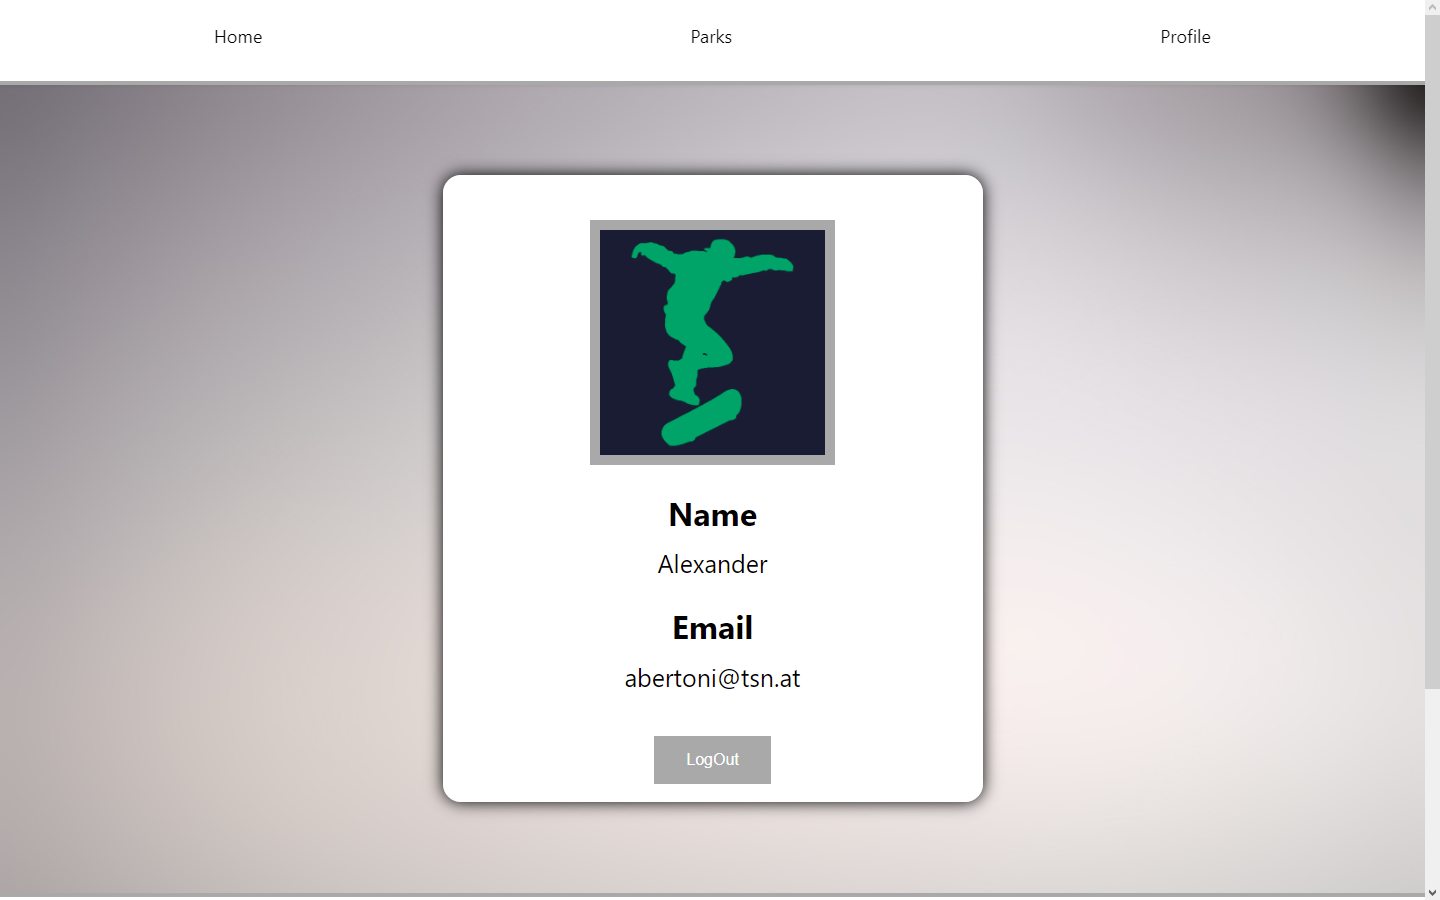
\includegraphics[width=1\textwidth]{Website/Profile.png}}
      \caption{Profil}
    \end{center}
\end{figure}

Auf der Profilseite ist es möglich seinen Benutzernamen und seine Email einzusehen. Außerdem ist es  
möglich sich von der Seite wieder auszuloggen. Die Informationen über den Benutzer werden ganz einfach über 
seinen token ausgelesen. Ist der Anwender auf der Seite nicht eingeloggt und er versucht auf die Profilseite
zu gelangen indem er die URL dieser Seite eingibt, leitet diese ihn auf die Login-view weiter. Die
Überleitung auf die Login view erfolgt wie folgt:

\begin{code}[htp]
\begin{lstlisting}
    useEffect(() => {
        if(!sessionStorage.getItem("data")){
            navigate("/LogIn");
        }
      });
\end{lstlisting}
\caption{React Component - Navigiert nach Login falls der Benutzer nicht eingeloggt ist}
\end{code}

UseEffect ist ein React Hook welcher ausgeführt wird, wenn die Seite einmal geladen wurde. Diese 
Überprüfung wird auch in der Admin-View der Seite verwendet um unerlaubten Zugriff zu vermeiden.